\documentclass{article}\usepackage{graphicx, color}
%% maxwidth is the original width if it is less than linewidth
%% otherwise use linewidth (to make sure the graphics do not exceed the margin)
\makeatletter
\def\maxwidth{ %
  \ifdim\Gin@nat@width>\linewidth
    \linewidth
  \else
    \Gin@nat@width
  \fi
}
\makeatother

\IfFileExists{upquote.sty}{\usepackage{upquote}}{}
\definecolor{fgcolor}{rgb}{0.2, 0.2, 0.2}
\newcommand{\hlnumber}[1]{\textcolor[rgb]{0,0,0}{#1}}%
\newcommand{\hlfunctioncall}[1]{\textcolor[rgb]{0.501960784313725,0,0.329411764705882}{\textbf{#1}}}%
\newcommand{\hlstring}[1]{\textcolor[rgb]{0.6,0.6,1}{#1}}%
\newcommand{\hlkeyword}[1]{\textcolor[rgb]{0,0,0}{\textbf{#1}}}%
\newcommand{\hlargument}[1]{\textcolor[rgb]{0.690196078431373,0.250980392156863,0.0196078431372549}{#1}}%
\newcommand{\hlcomment}[1]{\textcolor[rgb]{0.180392156862745,0.6,0.341176470588235}{#1}}%
\newcommand{\hlroxygencomment}[1]{\textcolor[rgb]{0.43921568627451,0.47843137254902,0.701960784313725}{#1}}%
\newcommand{\hlformalargs}[1]{\textcolor[rgb]{0.690196078431373,0.250980392156863,0.0196078431372549}{#1}}%
\newcommand{\hleqformalargs}[1]{\textcolor[rgb]{0.690196078431373,0.250980392156863,0.0196078431372549}{#1}}%
\newcommand{\hlassignement}[1]{\textcolor[rgb]{0,0,0}{\textbf{#1}}}%
\newcommand{\hlpackage}[1]{\textcolor[rgb]{0.588235294117647,0.709803921568627,0.145098039215686}{#1}}%
\newcommand{\hlslot}[1]{\textit{#1}}%
\newcommand{\hlsymbol}[1]{\textcolor[rgb]{0,0,0}{#1}}%
\newcommand{\hlprompt}[1]{\textcolor[rgb]{0.2,0.2,0.2}{#1}}%

\usepackage{framed}
\makeatletter
\newenvironment{kframe}{%
 \def\at@end@of@kframe{}%
 \ifinner\ifhmode%
  \def\at@end@of@kframe{\end{minipage}}%
  \begin{minipage}{\columnwidth}%
 \fi\fi%
 \def\FrameCommand##1{\hskip\@totalleftmargin \hskip-\fboxsep
 \colorbox{shadecolor}{##1}\hskip-\fboxsep
     % There is no \\@totalrightmargin, so:
     \hskip-\linewidth \hskip-\@totalleftmargin \hskip\columnwidth}%
 \MakeFramed {\advance\hsize-\width
   \@totalleftmargin\z@ \linewidth\hsize
   \@setminipage}}%
 {\par\unskip\endMakeFramed%
 \at@end@of@kframe}
\makeatother

\definecolor{shadecolor}{rgb}{.97, .97, .97}
\definecolor{messagecolor}{rgb}{0, 0, 0}
\definecolor{warningcolor}{rgb}{1, 0, 1}
\definecolor{errorcolor}{rgb}{1, 0, 0}
\newenvironment{knitrout}{}{} % an empty environment to be redefined in TeX

\usepackage{alltt}
\usepackage[round]{natbib}
\usepackage[nolists]{endfloat}
\usepackage[width = 5in]{geometry}
\usepackage{caption, amsmath, graphicx, setspace, multirow, color, hyperref, array}

%\renewcommand{\efloatseparator}{\mbox{}}

\newcommand\T{\rule{0pt}{2.6ex}}       % Top strut
\newcommand\B{\rule[-1.2ex]{0pt}{0pt}} % Bottom strut
\newcolumntype{x}[1]{%
>{\centering\hspace{0pt}}p{#1}}%

\defcitealias{Netherlands2004}{Netherlands, 2004}
\defcitealias{UNDESA2012}{United Nations, 2012}
\defcitealias{USFHA2012}{USFHWA, 2012}

\title{The Negative Effect of Traffic Noise on House Prices: A Landscape Hedonic Analysis}
\date{}

\doublespacing
\begin{document}
\maketitle
\pagenumbering{roman}
\begin{singlespace}
\begin{abstract}
One consequence of the expanding road network and its associated traffic is increased levels of traffic noise.  While the hedonic literature has consistently shown a negative effect of this phenomenon on the real estate market, research in the United States has often relied on crude measures of traffic noise. Here, we reduce the measurement error of traffic noise exposure through a detailed model of noise propagation over the landscape. Additionally, we estimate the impact on single family home transactions throughout the St.\ Paul, Minnesota, urban area using spatially explicit local regression techniques to allow for spatial non-stationarity in the hedonic function. Contrary to previous work, we find no evidence that the effect of traffic noise varies significantly across the several hundred square miles of our study region, nor by traffic noise levels. We do find significant differences in the impact of traffic noise before and after the economic recession of 2008-09. Our results suggest that an increase in traffic noise of one decibel decreases house prices by an average of 0.19 percent before September 2008 and an average of 0.37 percent after September 2008.
\end{abstract}
\end{singlespace}

\clearpage
\pagenumbering{arabic} 

\section{Motivation and Past Research}\label{sec:lit}
Prolonged exposure to traffic noise affects people in a number of ways, ranging from simple annoyance \citep{Miedema2001, Ouis2001, Ohrstrom2007, DeKluizenaar2013, Weinhold2013}, to sleep disturbance \citepalias{Netherlands2004}, to increasing risk for stroke \citep{Sorensen2011}, hypertension \citep{Jarup2008, Bodin2009}, myocardial infarction \citep{Babisch2005}, and overall quality of life \citep{Shepherd2013}. The noise level at which such effects are observed does not have to be high.  It has been shown that people exposed to traffic noise with a 24-hour average of 55 decibels (dBA) are found to be at a higher risk for hypertension \citep{Barregard2009, Bodin2009}, and those exposed to 60 dBA or greater are found to be at a higher risk for stroke \citep{Sorensen2011}.  

Automobiles are already perhaps the greatest source of noise in residential neighborhoods \citep{Barber2010} and traffic noise was estimated to cause around three billion dollars worth of external damage to the United States economy alone in 1991 \citep{Delucchi1998}. Traffic noise and its attendant problems are greater now than they were in the 1990s and predicted to worsen in the future \citep{Goines2007}.  %With the exception of a slight dip during the economic recession in the late 2000s, the number of vehicle miles traveled in the United States has steadily increased for the past 50 years.\footnote{\url{http://www.fhwa.dot.gov/policyinformation/statistics/2011/pdf/rc1c.pdf}} 
Globally, \citet{Dargay2007} predict the number of personal vehicles to grow from roughly 800 million in 2002 to over two billion units by 2030. Additionally, the global trend of increased urbanization is expected to continue, with the proportion of the population living in cities growing from roughly half now to over two-thirds by the middle of the century \citepalias{UNDESA2012}. 

One way to estimate some of the costs of traffic noise (and therefore the economic benefits of policies that reduce noise) is through hedonic regression, examining the relationship between house prices and noise levels. \citet{Nelson1982} was the first to review some of the earliest noise hedonic work in the United States and Canada. The review of nine studies found an average estimated impact of traffic noise to be a reduction in house prices of approximately 0.4 percent per additional decibel. More recently, \citet{Nelson2008} notes that many of these early studies \citep[such as][]{Gamble1974, Langley1976} are plagued by issues of small sample sizes (in the hundreds) and limited spatial extents (one or a handful of cities). 

Reviews of the research by \citet{Bateman2001} found that the negative effect of traffic noise on house prices ranged from 0.08 to 2.22 percent per decibel with a mean around 0.55 percent per decibel, while \citet{Navrud2002} found an average decrease of 0.64 percent per decibel. Much of the recent research in this literature has tended to focus on the European experience with noise, often due to the availability of high quality traffic noise data made available from the government, especially the United Kingdom \citep{Day2007, Blanco2011}, Sweden \citep{Wilhelmsson2000, Andersson2010}, Switzerland \citep{Baranzini2010}, Spain \citep{MarmolejoDuarteCarlos;GonzalezTamez2009}, Netherlands \citep{Theebe2004a}, and Germany \citep{Brandt2011}. 

Instead of focusing on the impact of automobile traffic noise, hedonic work in the United States has tended to concentrate on noise from airports \citep{Espey2000, McMillen2004, Cohen2008a} or indirect measures of traffic noise, such as proximity to highways \citep{Matthews2007, Chernobai2009, Li2012}, or traffic counts \citep{HughesJr.1992, Larsen2012}. One exception is \citet{Cheng2008}, which finds that an additional decibel of traffic noise reduced house prices in Louisville, Tennessee, by 0.34 percent during the year 2007. However, the generalizability of this research is limited given that it is based on less than a thousand house transactions in just one city. 

A major reason for the thinness of the scholarly literature on this topic in the US lies in the difficulty of modeling traffic noise propagation over the landscape. To properly analyze the spatial association between real estate prices and exposure to traffic noise, it is necessary to create a noise surface map at sufficiently detailed spatial resolution to account for the complex and heterogeneous interaction between the noise source and the resistance of the landscape to noise propagation.  Implementing such a model can be very difficult.  The data needed for the model is very extensive and may not even be readily available (e.g., building footprint and height data).  Furthermore, it is computationally very intensive. Fortunately, recent developments in Geographic Information Systems and distributive computing have reduced these difficulties, making it much easier to create a noise surface map at landscape level with high spatial resolution.  

In this paper, we estimate the relationship between traffic noise and single family house prices across 44 cities and several hundred square miles in the St.\ Paul, Minnesota, urban region by taking advantage of a uniquely detailed set of noise estimates. The data represent perhaps the most accurate regional noise estimates ever used in the hedonic literature in the United States to date due to the high spatial resolution of the estimates (10 m x 10 m) and the incorporation of the effects of nearby buildings and land cover on noise propagation. More detail about the noise model inputs and procedures are presented in the next section of the paper. 
 
%Precise estimates of the impact of traffic noise are important for efficient implementation of noise mitigation projects. The US Federal Highway Admistration reports that 47 states have constructed noise barriers to reduce noise propagation, spending over a half a billion dollars from 2008-2010 \citepalias{USFHA2012}. \citet{Delucchi1998} used an estimate of 0.85 percent reduction in house prices per additional decibel in their cost-benefit analysis of traffic noise. While their preferred estimate of the total damage cost to the United States in 1991 is \$3 billion, they report a possible range of less than \$100 million to over \$40 billion due in part to uncertainty surrounding the degree of noise propagation over space in the urban built environment and the effect of noise on house prices. Indeed, one of the main conclusions of their work is that more research should be done to better understand the impact of noise on house prices and that better noise data are needed for such work to occur. 

Work from Europe suggests that the relationship between traffic noise and house prices varies across housing submarkets \citep{Day2007, MarmolejoDuarteCarlos;GonzalezTamez2009}, by level of traffic noise \citep{Theebe2004a, Brandt2011}, and over time \cite{Wilhelmsson2000}. As such, we construct a flexible hedonic model that allows for a non-stationary relationship between house prices and our explanatory variables over geography and time. Such Locally Weighted Regression (LWR) models have become increasingly common in published work \citep[see][]{MarmolejoDuarteCarlos;GonzalezTamez2009, Carruthers2010, Sunding2010, Nappi-Choulet2011} and have been shown to be more accurate than other common spatial econometric models under common real world circumstances \citep{McMillen2012}. Thus, in addition to using new data that reduces the measurement error of the impact of traffic noise, the spatial and temporal variation in our data and hedonic modeling allow us to present the first estimates in the United States of how the impact of traffic noise varies over space, time, and by noise level. 

We find that while the impact of other important control variables in the hedonic function vary significantly over space, the impact of traffic noise does not. Such results are contradictory to recent work by \citet{MarmolejoDuarteCarlos;GonzalezTamez2009} which found evidence of a spatially non-stationary relationship between traffic noise and housing prices using a LWR model in Barcelona, Spain. Our paper also presents the first estimates of the implicit price of traffic noise after the housing market collapse and economic recession of 2008-09. Contrary to work such as \citet{Cho2011b}, which found that environmental amenities mattered \emph{less} after the housing crash, our estimated effect of traffic noise mattered \emph{almost twice as much more} after the recession (0.19 percent reduction in house prices per additional decibel beforehand compared to 0.37 percent per decibel afterwards). We conclude with a discussion of how future research can expand and improve upon this work.
 
\section{Study Area and Data}
The 2010 US Census lists the population of the Twin Cities Metropolitan Region (Minneapolis and St.\ Paul and their surrounding areas) as almost 3 million residents spread over seven counties. This study examines single family residential home transactions in the Census-defined urban areas of three of the seven counties: Dakota, Ramsey and Washington County (see Figure \ref{fig:overview}). We obtained sales data from approximately forty thousand transactions between 2005 and 2010 (n=42,095) from the 2010 MetroGIS Regional Parcel Dataset published by the Metropolitan Council. Figure \ref{fig:overview} shows an overview of the study area as well as the spatial distribution of the house sales prices. 

In addition to the geographic location and date of the house sale, we collected or calculated structural and locational variables commonly used in the hedonic literature, such as the size of the house, lot size, and architectural style of the house, as well as distances to amenities like the Central Business District, parks, and lakes. Table \ref{tab:sumStats} provides a brief description of the variables in our data and some basic summary statistics. Table \ref{tab:cor} displays a simple correlation matrix of the quantitative variables.

\begin{figure}
\makebox[\textwidth][c]{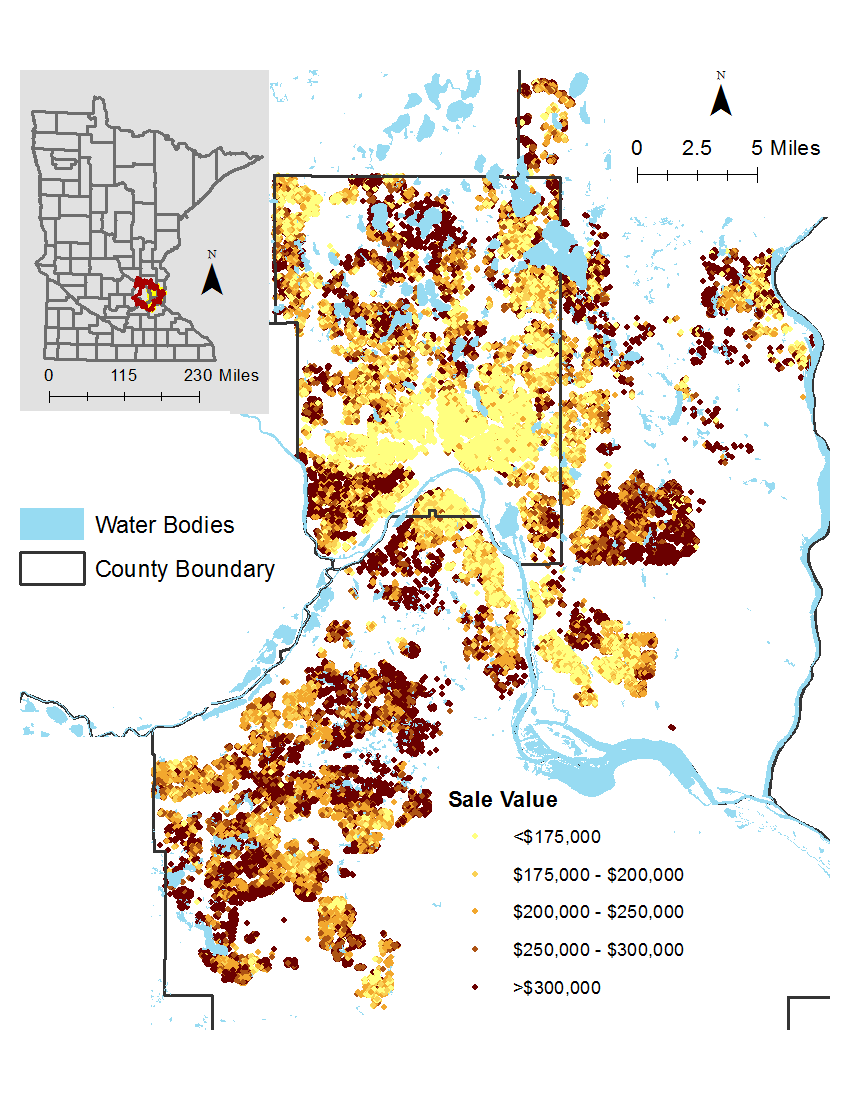
\includegraphics[width = 1.2\textwidth]{../graphs/StudyAreaSaleValueDist}}
\caption{This figure shows the spatial extent of our study area as well as the significant spatial variation in single family house sales prices.}\label{fig:overview}
\end{figure}

\begin{table}
\caption{Variable Description and Summary Statistics}\label{tab:sumStats}
\makebox[\linewidth][c]{
\small
\begin{tabular}{lrrrrrrr}
  
 & min & 25\% & 50\% & mean & 75\% & max & st.\ dev.\ \\ 
  \hline
  Sale Price (\$1,000s) & 98.8 & 195.0 & 241.0 & 265.5 & 314.9 & 675.0 & 102.8 \\ 
  House Size (square feet) & 390 & 1158 & 1628 & 1750 & 2188 & 4000 & 704 \\ 
  Lot Size (acres) & 0.02 & 0.17 & 0.25 & 0.25 & 0.31 & 0.60 & 0.11 \\ 
  Owner Occupancy (no = 0, yes = 1) & 0.0 & 1.0 & 1.0 & 0.8 & 1.0 & 1.0 & 0.4 \\ 
  Year of House Construction & 1850 & 1950 & 1973 & 1967 & 1993 & 2010 & 32 \\ 
  Traffic Noise (dB) & 25.1 & 50.5 & 55.3 & 56.4 & 62.2 & 91.5 & 8.8 \\ 
  Median Income in Census Tract (\$1,000s) & 13.9 & 54.6 & 69.1 & 72.6 & 89.7 & 143.3 & 23.6 \\ 
  Average 3rd Grade Standardized Test Scores & 335.6 & 359.8 & 365.4 & 364.5 & 370.4 & 551.7 & 10.6 \\ 
  Distance to Central Business District (km) & 1.1 & 6.8 & 13.2 & 14.7 & 21.8 & 37.1 & 8.9 \\ 
  Distance to nearest Park (km) & 0.0 & 1.1 & 2.2 & 2.6 & 3.8 & 9.7 & 1.9 \\ 
  Distance to nearest Lake (km) & 0.0 & 0.4 & 0.8 & 0.9 & 1.3 & 4.4 & 0.7 \\ 
  Distance to nearest Shopping Center (km) & 0.0 & 0.9 & 1.5 & 1.9 & 2.3 & 10.8 & 1.6 \\ 
   \hline
\end{tabular}
}
\end{table}

\begin{table}
\caption{Matrix of Pearson Correlation Coefficients for Quantitative Variables}\label{tab:cor}
%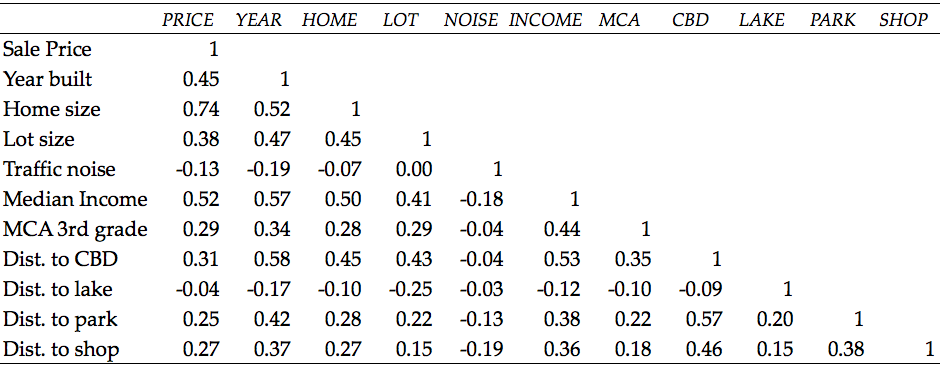
\includegraphics[width = \textwidth]{../graphs/CorrelationMatrix}
\begin{center}
\small
\tabcolsep=0.05cm
\makebox[\linewidth][c]{
\begin{tabular}{l|rrrrrrrrrrr}
 & \multicolumn{1}{x{.35in}}{Price} & \multicolumn{1}{x{.38in}}{House} & \multicolumn{1}{x{.35in}}{Lot} & 
 \multicolumn{1}{x{.35in}}{Built} & \multicolumn{1}{x{.35in}}{Noise} & \multicolumn{1}{x{.35in}}{Inc.} & 
 \multicolumn{1}{x{.35in}}{Test} & \multicolumn{1}{x{.35in}}{CBD} & \multicolumn{1}{x{.35in}}{Park} & \multicolumn{1}{x{.35in}}{Lake} & \multicolumn{1}{x{.35in}}{Shop} \tabularnewline 
  \hline
Sale Price & 1 &  &  &  &  &  &  &  &  &  &  \tabularnewline 
  House Size & 0.74 & 1 &  &  &  &  &  &  &  &  &  \tabularnewline
  Lot Size & 0.38 & 0.45 & 1 &  &  &  &  &  &  &  &  \tabularnewline
  Year Built & 0.45 & 0.52 & 0.47 & 1 &  &  &  &  &  &  &  \tabularnewline
  Noise & -0.13 & -0.07 & 0.00 & -0.19 & 1 &  &  &  &  &  &  \tabularnewline
  Income & 0.52 & 0.50 & 0.41 & 0.57 & -0.18 & 1 &  &  &  &  &  \tabularnewline
  Elem.\ Test Scores & 0.29 & 0.28 & 0.29 & 0.34 & -0.04 & 0.44 & 1 &  &  &  &  \tabularnewline 
  Distance to CBD & 0.31 & 0.45 & 0.43 & 0.58 & -0.04 & 0.53 & 0.35 & 1 &  &  &  \tabularnewline
  Distance to Park & 0.25 & 0.28 & 0.22 & 0.42 & -0.13 & 0.38 & 0.22 & 0.57 & 1 &  &  \tabularnewline
  Distance to Lake & -0.04 & -0.10 & -0.25 & -0.17 & -0.03 & -0.12 & -0.10 & -0.09 & 0.20 & 1 &  \tabularnewline
  Distance to Shop & 0.27 & 0.27 & 0.15 & 0.37 & -0.19 & 0.36 & 0.18 & 0.46 & 0.38 & 0.15 & 1 \tabularnewline
\end{tabular} }
\end{center} 
\end{table}

\subsection{Noise Data}
To determine the relationship between real estate price and road traffic noise levels, we first created a traffic noise exposure surface by calculating the propagation of traffic noise over the landscape using the FHWA (Federal Highway Authority) 1978 standard \citep{Barry1978}. Following \citet{Barry1978}, the traffic noise level at any given location on the landscape is given by: 
\begin{eqnarray}\label{eq:noise}
L_{EQ}(i) &=& \bar{L}_0(i) + 0.115 \sigma _i^2 + 10 log \frac{N_i \pi D_0}{T*S_i} + 10 log \left[ \frac{D_0}{D}\right]^{1 + \alpha}  \nonumber \\
&& + 10 log \left( \frac{\psi _{\alpha (\phi _1, \phi _2)}}{\pi}\right) + \Delta _{gradient} + \Delta _{shielding}
\end{eqnarray}
where $L_{EQ}(i)$ is A-weighted hourly energy equivalent noise level in decibels (dBA), which is calculated for each class $i$ of vehicle (automobile and trucks); $\bar{L}_0(i)$ is the mean Sound Pressure Level (SPL) at the reference distance for class $i$; $\sigma _i$ is the standard deviation of the SPL for each class of vehicle; $N_i$ is the number of vehicles of the $i^{th}$ class passing during the relevant hour; $D_0$ is the reference distance (usually 15 m); $D$ is the perpendicular distance from the road center line to the receiver; $\alpha$ is a site parameter (soft and hard surface), $0 < \alpha < 1$; $S_i$ is the mean speed of the $i^{th}$ class; $T$ is the duration, usually 1 hour; $\phi _1$ and $\phi _2$ are the angles from the perpendicular of the limits of the observer's view of a section of the road. They are used to account for only the energy coming from a portion of the roadway; $\Delta _{gradient}$ is an adjustment for road surface gradient; $\Delta _{shielding}$ is a shielding adjustment (land cover, buildings, noise barriers).

To calculate the traffic noise map for the region using the above model, several data sources were used. A 2007 road centerline and the associated traffic characteristics (volume and proportion of trucks and vehicles) for the region were obtained from the Minnesota Department of Transportation (MNDoT). We converted the posted speed of each road into a GIS layer. For all roads without recorded traffic volume (i.e., residential), we assigned 100 vehicles/day as a minimum estimate. This estimate was based on factors identified in the literature as important for estimating traffic volume, such as census data on commuting population, tract area, the size of a standard street block, and road type \citep{Cheng1992, Fricker1986}.\footnote{In order to assess the sensitivity of our results to our estimate of traffic volume for local roads, we also ran the model using 200 and 300 vehicles/day for one county. With the exception of a few areas in the rural part of the county, there was less than 0.05 dBA difference at 30 m from the road centerline.}

Data on traffic volume and the proportion of trucks and vehicles on each segment of the road were averaged over a 24-hour period, making it impossible to account for a day and night time variation in traffic noise. Following \citet{Arditi2007}, we divided the total traffic volume into day and nighttime periods by assuming that 80 percent of vehicles and 65 percent of trucks are driven during the daytime (6am -- 10pm) and 35 percent of trucks and 20 percent of vehicles are driven during the nighttime (10pm--6am). Values for ground absorption were chosen by assuming that all road surfaces consisted of impervious bitumen. For computational simplicity, we created the road surface gradient by re-sampling US Geological Survey 30 m resolution Digital Elevation Model (DEM) to 100 m resolution. 

We used three data sources for the shielding adjustment: buildings, foliage, and noise barriers. We extracted the perimeter and height of 818,500 buildings using aerial photography and LiDAR data. For the areas where LiDAR data are available, we used LiDAR Analyst$^{TM}$ software to extract buildings’ footprints. For the areas of the region where only aerial photos are available, we used Feature Analyst$^{TM}$ software to extract building footprints. For measurements extracted using aerial photography, height was determined using a combination of parcel data and field measurements. 

The locations chosen for the traffic noise levels were the 818,500 buildings in the entire urban area. Thus, we used the perimeter and height of these buildings to account for the shielding effect of buildings. To account for foliage shielding (and to make the computation manageable), we assumed that only forest patches that are at least 10 m high and have an area greater than 10,000 m$^2$ will have a significant effect on noise attenuation. Accordingly, we extracted forest polygons with these characteristics using a combination of year 2005 land use data and 2001 National Land Cover Data (NLCD). To account for noise barrier shielding, we used a noise barrier layer obtained from MNDoT, which contains the locations, width, and height of noise barriers in the region.

We used the SoundPlan$^{TM}$ noise modeling software to implement the model given by Equation~\eqref{eq:noise}. Predicted traffic noise output is calculated at a grid resolution of 10 m$^2$.\footnote{We conducted a preliminary validation of the model output by comparing it with observed noise levels at 134 locations that were sampled along major highways. For each location, two readings were taken very close to the highway, one between 9am and 10am and another between 1pm and 2pm. The noise level for each location is then determined by averaging the two observed values, and this average is then compared with the predicted noise level. The relationship between the mean observed and predicted noise levels is linear and moderately strong with a correlation of 0.76. It is not surprising that the relationship is not stronger given the size and complexity of the model. In particular, the traffic volume data that we used for modeling traffic noise propagation is a 24-hour average, which requires more time-interval sampling per location than just the two used in the validation. Still, this preliminary comparison serves as a good indicator of how well this model captures traffic noise levels.} Once the noise surface for the entire region was developed, we extracted the noise surface for the present study area by overlaying the housing parcel boundaries and calculating the maximum noise level within the parcel.

\subsection{Structural Attributes}
According to a review by \cite{Wilhelmsson2000}, the five most common structural attributes included in real estate hedonic pricing studies are living area, number of bathrooms, age, garage and lot size.  The 2010 MetroGIS Regional Parcel Dataset includes structural data on living area, age, garage presence, lot size, owner-occupancy and house architectural style for every transaction. However, standard additional control variables like the number of bathrooms, bedrooms, and size of garage were not available through this source. We were able to obtain additional data for the number of bedrooms, bathrooms, and size of the garage for a subset of our house sales from the Dakota County Assessor's Office. In section \ref{Discussion} we show that the inclusion of these variables in our model does not significantly change our results for these areas. Therefore, we feel confident in our results even without these independent variables for most of our study area. %Additionally, other hedonic work has been published using a similar set of explanatory variables in this area, see for instance, \citet{Sander2009b}.

\subsection{Other Locational Attributes}
A common real estate adage states that the three most important real estate attributes are: location, location and location. Knowing where each house is located allows us to also construct a vector of other attributes associated with the sales transaction. For instance, using GIS software we are able to calculate the Euclidean distance to numerous points of interest within the dataset, such as the nearest central business district, shopping centers, parks, and lakes. Additionally, a variable denoting the median household income for the surrounding census tract is created through the use of TIGER shapefiles from the 2010 Census Bureau and data from the 2010 American Community Survey. Lastly, we associate each transaction with its elementary school and include the average 3rd grade Minnesota Comprehensive Assessment (MCA) score for the local elementary school during the year of purchase.\footnote{Test scores were obtained from the Minnesota Department of Education website. The school district and elementary school attendance boundary spatial information were obtained from the Minnesota Geospatial Information Office Clearinghouse Data Catalog.} 

\subsection{Time}
Given that we have data from before and after the recession of 2008-09, we subset the data in Table \ref{tab:SumStatsTime} by year of sale to look for differences over time. In addition to the noticeable decline in nominal sales values, there is also a drop in the number of sales across years. For example, in 2010 there were only 4,206 property sales within the dataset, less than half as many in 2005. While the mean sale price declined from roughly \$280,000 pre-crash to \$230,000 post-crash, most of the structural and neighborhood variables are relatively consistent across years. However, traffic noise displays a noticeable difference in the pre- and post-crash market transactions (the mean drops from over 58 dB to less than 53 dB). 

\begin{table}
\begin{center}
\caption{Mean Variable Values by Year}\label{tab:SumStatsTime}
\small
%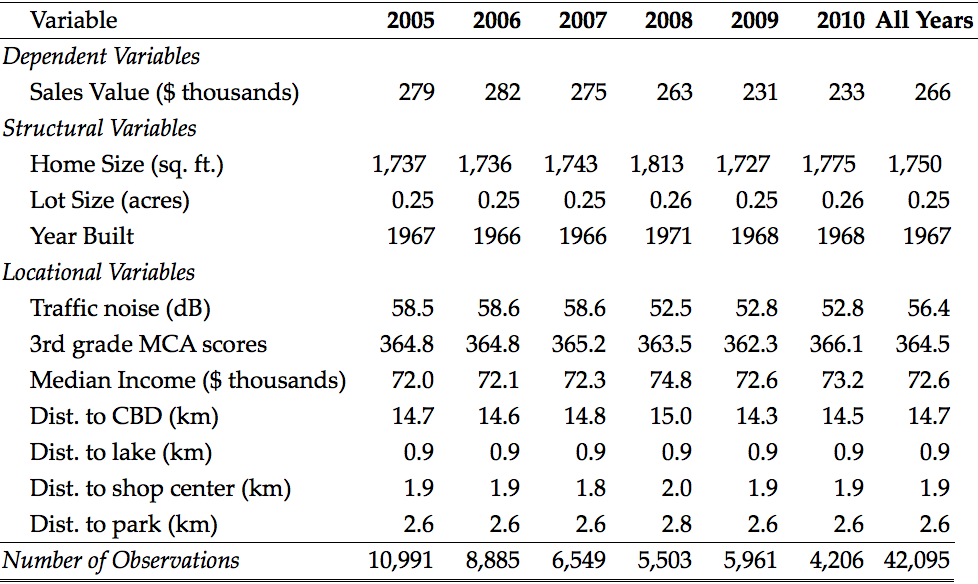
\includegraphics[width = \textwidth]{../graphs/DescriptiveStatsByYear}
% Table generated by Excel2LaTeX from sheet 'Descriptive StatisticsYear'
    \begin{tabular}{lrrrrrr|r}
    Variable & 2005 & 2006 & 2007 & 2008 & 2009 & 2010 & 2005-10\\ \hline
    Sales Value (\$1000s) & 279   & 282   & 275   & 263   & 231   & 233   & 266 \\
    Traffic Noise (dB) & 58.5  & 58.6  & 58.6  & 52.5  & 52.8  & 52.8  & 56.4 \\
    House Size (ft$^2$) & 1737  & 1736  & 1743  & 1813  & 1727  & 1775  & 1750 \\
    Lot Size (acres) & 0.25  & 0.25  & 0.25  & 0.26  & 0.25  & 0.26  & 0.25 \\
    Year Built  & 1967  & 1966  & 1966  & 1971  & 1968  & 1968  & 1967 \\
    Median Income (\$1000s) & 72.0  & 72.1  & 72.3  & 74.8  & 72.6  & 73.2  & 72.6 \\
    Elem. Test Scores & 364.8 & 364.8 & 365.2 & 363.5 & 362.3 & 366.1 & 364.5 \\
    Dist.\ to CBD (km) & 14.7  & 14.6  & 14.8  & 15.0  & 14.3  & 14.5  & 14.7 \\
    Dist.\ to Park (km) & 2.6   & 2.6   & 2.6   & 2.8   & 2.6   & 2.6   & 2.6 \\
    Dist.\ to Lake (km) & 0.9   & 0.9   & 0.9   & 0.9   & 0.9   & 0.9   & 0.9 \\
    Dist.\ to Shop (km) & 1.9   & 1.9   & 1.8   & 2.0   & 1.9   & 1.9   & 1.9 \\ \hline
    Number of Observations &  10,991  & 8,885  &  6,549  & 5,503  &  5,961  & 4,206  & 42,095  \\
    \end{tabular}%
\end{center}
\end{table}

\section{Basic Econometric Model}\label{basicModel}
Our aim is to estimate the marginal willingness to pay for different attributes, in particular changes in the traffic noise associated with the house. Consistent with past research, this study implements a semi-logarithmic hedonic pricing model.  Before implementing the Locally Weighted Regression model, we present the results of a simpler econometric model given by equation~\eqref{eq:model}.
\begin{equation}\label{eq:model}	
ln \textrm{ Sale Price}_i = \beta _0 + \beta _1 \textrm{Noise}_i+ \beta _2 S_i+ \beta _3 N_i + \beta _4 T_i + \textrm{error}_i
\end{equation}
Noise$_i$ is the noise level for house $i$, $S_i$ is a vector of the house's structural attributes, $N_i$ is a vector of the neighborhood attributes, and $T_i$ is a vector of time fixed effects. Due to the semi-logarithmic functional form of the model, we can interpret the regression model coefficients as the price semi-elasticities of the underlying attributes. For instance, we can interpret the coefficient on noise as the percentage increase in price for a one decibel increase in the traffic noise associated with the transaction in our dataset. 

\begin{table}
\caption{Basic Regression Results (dependent variable = $ln(\textrm{Sale Price})$)}\label{tab:globalRegression}

\makebox[\textwidth][c]{%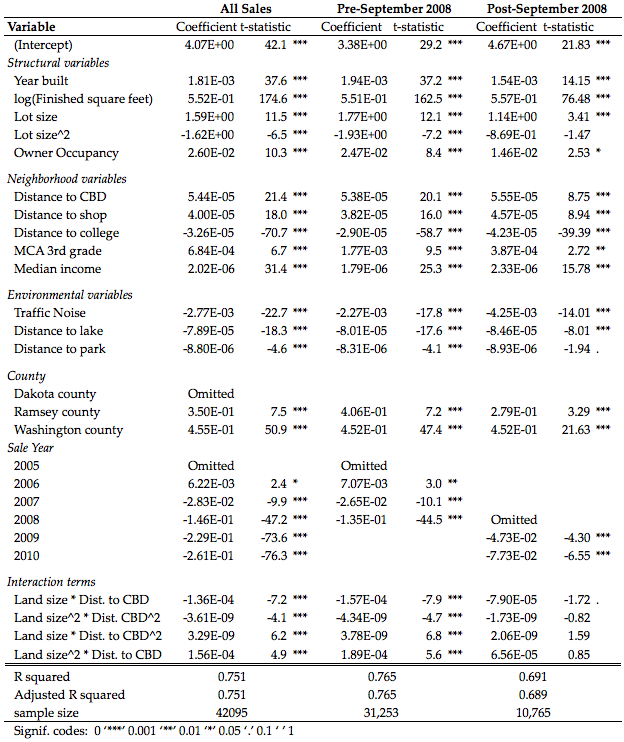
\includegraphics[width = 1.3\textwidth]{../graphs/GlobalRegression}}
% Table generated by Excel2LaTeX from sheet 'Sheet1'
  \centering
  \tabcolsep=0.03cm
    \begin{tabular}{lclcclcclccl}
   & (1)   &       &       & (2)   &       &       & Pre-Crash   &       &       & Post-Crash   &  \\ \hline
\T  Traffic Noise & -2.02E-03 & *** &   & -2.00E-03 & ***   &   & -1.63E-03 & ***  & & -3.08E-03 & *** \\
          & (1.32E-04) &   &   & (1.32E-04) &       &       & (1.38E-04) &       &       & (3.29E-04) &  \\
\T  Intercept & 9.37E+00 & ***   & \hspace{.5cm} & 9.49E+00 & ***   & \hspace{.5cm}   & 8.55E+00 & ***   & \hspace{.5cm}   & 1.10E+01 & *** \\
          & (9.48E-02) &    &   & (9.62E-02) &   &   & (1.11E-01) &       &       & (2.12E-01) &  \\
\T   House Size & 3.38E-04 & ***   &   & 3.39E-04 & ***   &   & 3.35E-04 & ***   &   & 3.50E-04 & *** \\
          & (1.85E-06) &   &   & (1.86E-06) &       &       & (1.99E-06) &       &       & (4.26E-06) &  \\
\T  Lot Size & 1.42E-01 & ***   &    & 2.74E-01 & ***   &   & 2.31E-01 & ***   &      & 2.74E-01 & *** \\
          & (1.14E-02) &     &   & (2.12E-02) &     &      & (2.29E-02) &       &       & (4.99E-02) &  \\
\T  Owner Occupancy & 3.22E-02 & ***   &   & 3.23E-02 & ***   &     & 3.38E-02 & ***  & & 2.61E-02 & *** \\
          & (2.80E-03) &  &   & (2.79E-03) &       &       & (3.24E-03) &       &       & (6.41E-03) &  \\
\T  Year Built & 7.82E-04 & ***   &   & 7.17E-04 & ***   &    & 9.68E-04 & ***   &   & 2.15E-06 &  \\
          & (4.57E-05) &       &       & (4.65E-05) &   &   & (5.06E-05) &    &   & (1.05E-04) &  \\
\T  Median Income & 3.03E-06 & ***  & & 3.31E-06 & ***  &   & 2.86E-06 & ***   &       & 4.06E-06 & *** \\
          & (5.87E-08) &       &       & (5.87E-08) &   &   & (6.56E-08) &       &       & (1.35E-07) &  \\
\T  Elem. Test Scores & 1.88E-03 & *** &   & 1.81E-03 & ***   &   & 3.11E-03 & *** & & 1.21E-03 & *** \\
          & (1.06E-04) &  &   & (1.06E-04) &   &       & (1.75E-04) &       &       & (1.55E-04) &  \\
\T  Distance to CBD & -1.56E-06 & ***  &  & 7.46E-07 & *     &  & -1.57E-07 &   &       & 1.40E-06 &  \\
          & (1.97E-07) &       &       & (3.70E-07) &       &       & (3.95E-07) &   &   & (8.98E-07) &  \\
\T  Distance to Park & -2.38E-07 &   &    & -5.48E-07 &    &   & -6.37E-07 &  &   & -4.01E-07 &  \\
          & (6.82E-07) & &   & (6.83E-07) &       &       & (7.33E-07) &       &       & (1.58E-06) &  \\
\T  Distance to Lake & 2.12E-05 & ***   &   & 2.36E-05 & ***   &   & 2.22E-05 & ***   & & 2.79E-05 & *** \\
          & (1.68E-06) &       &    & (1.71E-06) &   &    & (1.83E-06) & &  & (4.03E-06) &  \\
\T  Distance to Shop & 3.01E-06 & ***   &    & 3.12E-06 & ***   & & 4.16E-06 & ***   &    & 1.88E-06 &  \\
          & (7.67E-07) &       &       & (7.66E-07) &       &       & (8.17E-07) &  & & (1.82E-06) &  \\
\T  Lot Size * Distance to CBD &  &   & & -8.81E-06 & *** & & -6.66E-06 & ***   &       & -9.55E-06 & ** \\
          &   &   &   & (1.19E-06) &       &       & (1.27E-06) &       &       & (2.94E-06) &  \\
\T  County Fixed Effects & yes   &   &   & yes   &       &       & yes   &       &       & yes   &  \\
    Year of Sale Fixed Effects & yes   &   &   & yes   &   &       & yes   &       &       & yes   &  \\
    Month of Sale Fixed Effects & yes   &   &   & yes   &   &       & yes   &       &       & yes   &  \\ \hline
\T  Number of Observations &        42,095  &   &  &    42,095  & & &   31,253  & & &    10,842  &  \\
    R$^2$   & 0.696 &       &       & 0.696 &       &       & 0.714 &       &       & 0.613 &  \\
 \multicolumn{12}{l}{(standard errors) ***$p<.001$; **$p<.01$; *$p<.05$}  \\
    \end{tabular}%
}
\end{table}

Column (1) in Table \ref{tab:globalRegression} displays the results of our basic regression model. All coefficients but one are significantly different from zero at conventional significance levels. The traffic noise coefficient suggests that a one decibel increase traffic noise is on average associated with a 0.2 percent reduction in housing sales prices. Standard urban economic theory \citep{Alonso1964, Mills1967, Muth1969} predicts that the price of land will vary over space within our dataset to account for locational amenities. As such, the other columns include an interaction term between lot size and distance to the nearest central business district to account for spatial variation in the price of land. The significant coefficients on the lot size interaction terms suggest that the value of land varies over space. Other regressions (results available upon request) show similar variation in the implicit prices of house characteristics over space.

Table \ref{tab:globalRegression} also attempts to begin to understand how the economic recession may have influenced the hedonic function in our study area. The third and fourth columns estimate the same regression as (2) but subset the sales before and after September of 2008 (the month that Lehman Brothers filed for bankruptcy, the US Federal government took over Fannie Mae and Freddie Mac, and the American International Group (AIG) narrowly avoided bankruptcy only through a \$85 billion loan from the US Federal government).\footnote{\url{http://www.federalreserve.gov/newsevents/press/other/20080916a.htm}} The coefficients for some of the hedonic variables of interest (noise, schools, land, for instance) appear different across the two time periods.

The results in Table \ref{tab:globalRegression} and previous work \citep[such as][]{Day2007, MarmolejoDuarteCarlos;GonzalezTamez2009} suggests that the relationship between prices and many other hedonic characteristics may vary over space. While methods exist for parameterizing this variation \citep[such as spatial expansion as suggested by][]{Casetti1972}, we have no a priori knowledge of how to parameterize the variation over space and time. As such, we turn to a semi-parametric form of hedonic regression, a flexible modeling approach which lets the data reveal how relationships vary, rather than specifying them beforehand. Such a modeling choice will allow us to test the hypotheses of spatial and temporal stationarity in the regression model.

\section{Locally Weighted Regression Model}
Locally Weighted Regression (LWR) techniques (also known as Geographically Weighted Regression) are described in detail by \citet{Cleveland1988}, \citet{Brunsdon1998b}, \citet{Fotheringham2002}, and others. It is a weighted least squares methodology in which regression coefficients are estimated over space as a function of the local data as described in Equation~\eqref{eq:LWRbeta},
\begin{equation}\label{eq:LWRbeta}
\hat{\beta}_i = (X'W_iX)^{-1}X'W_iY,
\end{equation}
where X is a $n \times m$ matrix of independent variables, $W_i$ is the $n \times n$ weights matrix, and Y is the $n \times 1$ vector of dependent variable values. The weights matrix, $W_i$ is a diagonal matrix where element $w_{jj}$ denotes the weight that the $j^{th}$ data point will receive in the regression coefficients estimated at location $i$ in the dataset. We employ a bi-square weights function and a k-nearest neighbor bandwidth approach as described in equation~\eqref{eq:weights}, 
\begin{equation}\label{eq:weights}
w_{jj}=\left[1-\left(\frac{d_{ij}}{d_{k}}\right)^2 \right]^2 \textrm{ if  }d_{ij}<d_{ik}\textrm{, otherwise = 0},
\end{equation}
where $d_{ij}$ denotes the distance between observations $i$ and $j$, and $d_{ik}$ is the distance from observation $i$ to the $k^{th}$ nearest observation. This function assigns weights close to 1 for data points near observation $i$, weights positive but closer to zero for observations farther away, and zero for all $n-k$ observations farther away than the $k^{th}$ nearest observation. We estimate LWR coefficients using bandwidths ranging from as small as $k=50$ observations and as large as 10,000 observations. We choose the LWR bandwidth my minimizing the Generalized Cross Validation score as detailed in equation~\eqref{eq:GCV},
\begin{equation}\label{eq:GCV}
n*\sum_{i=1}^{n}\frac{(y_i-\hat{y}_i)^2}{(n-v_1)^2}, 
\end{equation} 
where $y_i$ is the dependent variable value, $\hat{y}_i$ is the predicted dependent variable value for observation $i$, and $v_1$ is the ``effective number of model parameters.''
$v_1=$tr(\textbf{S}), where the matrix \textbf{S} is the ``hat matrix'' which maps $y$ onto $\hat{y}$,
                   \begin{equation*}
                   \hat{y}=\textbf{S}y,
                   \end{equation*}
                   and each row of \textbf{S}, $r_i$ is given by:
                     \begin{equation*}
                   r_i=X_i(X'W_iX)^{-1}X'W_i.
                   \end{equation*}
The GCV score is a convenient model selection metric that rewards models that provide a good fit to the data, while penalizing models with a greater number of model parameters \citep{Loader1999, McMillen2010}. Model selection via this strategy has been shown to discern whether spatially varying relationships exist, accurately estimate spatially varying coefficients, even outperform other spatial econometric techniques, and do so without wasting degrees of freedom \citep{Paez2011, McMillen2010, McMillen2012}. 

%\section{Results}
Similar to the basic econometric model described in Section \ref{basicModel}, the LWR model estimates the logged sales price of a house as a function of structural variables, location and time. In order to account for changing market conditions in our data, when estimating LWR coefficients we use only houses sold within the past 12 months. Thus, the coefficient estimates at a particular house are estimated using data from other sales nearby in both time and geography.

\subsection{Improved Model Performance}
The use of the Locally Weighted Regression model significantly increases model performance. Figure \ref{fig:GCVmodel} displays the Generalized Cross Validation score for three different model specifications with varying number of observations included in the regression bandwidth. Two important conclusions can be drawn from the results. First, local analysis (bandwidths of a couple hundred observations) perform significantly better than global models, and second, conditional on the bandwidth, performance improves with the inclusion of more locational variables. The minimum GCV score is obtained using a bandwidth of 200 nearest houses and a model including structural, locational, and city fixed-effects.

We estimate three different models. Model (1) uses only the basic structural characteristics as the explanatory variables (size of the house in square feet, size of the lot in acres, a categorical variable denoting the architectural style of the house, and whether or not the house is owner-occupied). Model (2) adds locational variables to the previously described model (test scores at the local elementary school, census tract median income, and distances to the central business district, nearest park, nearest shopping center, and nearest lake). The third model adds city fixed effects. Generally speaking, the third model performs slightly better than the second model, which performs substantially better than the first model. 
\begin{figure}
  \makebox[\textwidth][c]{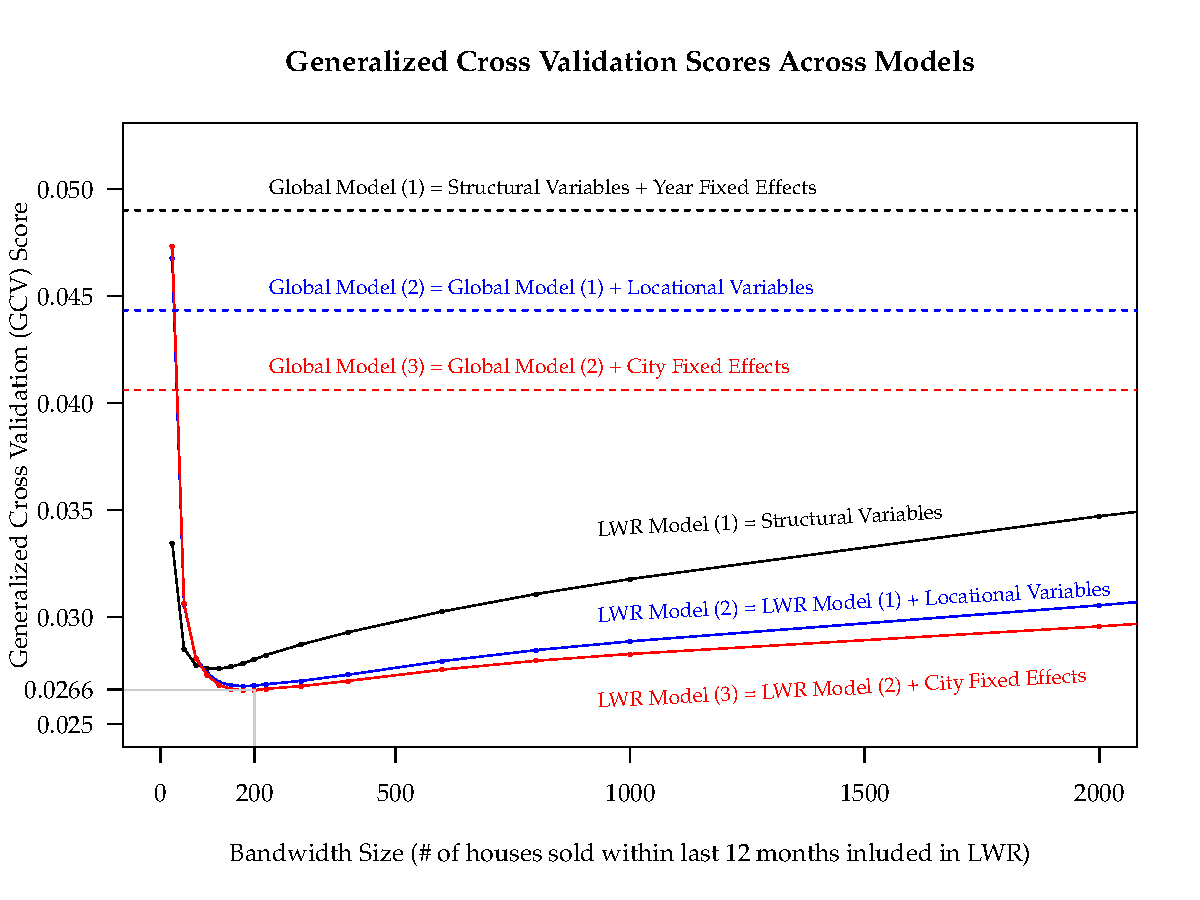
\includegraphics[width = 1.2\textwidth]{../graphs/GCVbyModel}}
\caption{This figure shows the relationship between bandwidth size and the GCV score for three different Locally Weighted Regression (LWR) models. For comparison, the GCV scores for each model when estimated at a global scale are also shown. Note that the LWR models all have significantly smaller GCV scores than the global models. The minimum GCV score is obtained by LWR Model (3) at a bandwidth of 200 nearest houses.}\label{fig:GCVmodel}
\end{figure}

We also estimate each of the three models at varying levels of local analysis, with bandwidths ranging from the nearest 50 observations to the nearest 10,000. Models with bandwidths of only a couple hundred observations have substantially smaller GCV scores, suggesting that, conditional on control variables included in the model, model performance still improves by performing the analysis at the local level. It is also worth noting that the LWR models have significantly lower GCV scores for a range of bandwidths when compared to the global models. These results suggest that it is important to model our data in a spatially explicit manner. 

Table \ref{tab:mainresults} displays a summary of the results of LWR Model (3) and a similar regression model run without allowing for spatial variation in the regression coefficients. Again, note that the LWR model yields a substantially smaller GCV score (0.027 vs.\ 0.041) signifying a substantial improvement in model performance. In addition to the significant reduction in the GCV score obtained with the use of LWR, we also see a substantial reduction in the degree of spatial autocorrelation in the model residuals. We calculate Moran's I statistic to be 0.199 for the global model while our preferred LWR specification yields 0.012, a more than ten-fold reduction. 

% latex table generated in R 2.15.2 by xtable 1.7-0 package
% Mon Jun 24 16:36:58 2013

\begin{table}[bp]
\caption{Hedonic Regression Results (dependent variable = $ln(\textrm{Sale Price})$)} \label{tab:mainresults} 
\makebox[\linewidth]{
\small
\begin{tabular}{lrrrrrr} \\
 & \multicolumn{2}{c}{Global Model} & \multicolumn{4}{c}{Locally Weighted Regression Model} \\
 & \multicolumn{1}{c}{$\hat{\beta}$} & \multicolumn{1}{c}{$\hat{\sigma}_{\hat{\beta}}$} & mean $\hat{\beta}$ & \multicolumn{1}{c}{$\sigma_{\hat{\beta}}$} & (5) & (6) \\ 
  \hline
(Intercept) & 8.4E+00 & 1.3E-01 & 2.9E+00 & 1.5E+01 & 0.64 & 0.00 \\ 
  Traffic Noise & -2.6E-03 & 1.6E-04 & -2.5E-03 & 3.0E-03 & 0.47 & 0.67 \\ 
  House Size & 3.0E-04 & 2.7E-06 & 2.6E-04 & 9.1E-05 & 1.00 & 0.00 \\ 
  Lot Size & 2.6E-01 & 1.5E-02 & 4.0E-01 & 3.7E-01 & 0.67 & 0.00 \\ 
  Year Built & 1.2E-03 & 6.5E-05 & 4.5E-03 & 5.4E-03 & 0.79 & 0.00 \\ 
  Owner Occupancy & 2.7E-02 & 3.2E-03 & 2.3E-02 & 6.4E-02 & 0.37 & 1.00 \\ 
  Elem.\ Test Scores & 1.5E-03 & 1.2E-04 & 2.4E-04 & 3.1E-02 & 0.30 & 0.00 \\ 
  Median Income & 3.3E-06 & 7.7E-08 & 9.6E-07 & 8.1E-06 & 0.35 & 0.00 \\ 
  Dist.\ to CBD & 1.3E-05 & 6.3E-07 & 1.1E-05 & 1.0E-04 & 0.30 & 0.00 \\ 
  Dist.\ to Park & -3.7E-07 & 1.1E-06 & -1.6E-05 & 1.3E-04 & 0.32 & 0.00 \\ 
  Dist.\ to Lake & 2.5E-05 & 2.1E-06 & -2.8E-05 & 1.4E-04 & 0.35 & 0.00 \\ 
  Dist.\ to Shop & -5.3E-06 & 1.3E-06 & 1.5E-05 & 8.8E-05 & 0.29 & 0.00 \\  
  Location of Sale & \multicolumn{2}{c}{city fixed effects} & \multicolumn{4}{c}{\footnotesize city fixed effects and nearest 200 sales} \\
  Timing of Sale & \multicolumn{2}{c}{year fixed effects} & \multicolumn{4}{c}{within last 12 months} \\
 \hline
  GCV score & \multicolumn{2}{c}{0.041} & \multicolumn{2}{c}{0.027}  &  & \\
  Moran's I statistic & \multicolumn{2}{c}{0.199} & \multicolumn{2}{c}{0.012} & & \\
\end{tabular}
}
 \caption*{\footnotesize Column (5) displays the proportion of $\hat{\beta}_{LWR}$ that can reject the null hypothesis of $\beta =0$.\\ Column (6) displays the proportion of Monte Carlo simulations with larger standard deviations of the LWR coefficients than $\sigma_{\hat{\beta}}$}
\end{table}

The first two columns of Table \ref{tab:mainresults} display the estimates and standard errors from a basic semi-log OLS regression with traffic noise, structural characteristics, location-based amenities, and both city and year of sale dummy variables. The third and fourth columns summarize the results of the LWR model when coefficients are estimated at each observation within the dataset using the nearest 200 house sales within the past 12 months. The third column presents the mean of these estimates while the fourth column displays the standard deviation of the estimates to give a measure of variation in the estimates across the dataset. Most of the mean LWR coefficients, including traffic noise, are similar to the coefficients obtained with the global OLS model. However, the large standard deviations of the LWR coefficients suggest non-stationarity in the estimated coefficients with the more flexible model. We now try to determine the source of this variation.

Column (5) in Table \ref{tab:mainresults} shows the percentage of the local regressions for which the coefficient's p-value is less than 0.1. All regressions contained statistically significant estimates of the impact of increased living space and a majority contained significant estimates for lot size and year of construction. Roughly half of the regressions estimated an impact of traffic noise statistically different from zero, while approximately one-third of the local regressions estimated statistically significant estimates of the locational variables (school test scores, census tract median income, distance to local amenities). The lack of statistical significance for many of the local regression coefficients could be due to multiple factors. First, because we are estimating local regressions with only the nearest 200 data points, rather than tens of thousands of sales as in the global model, we might be estimating the coefficients with less precision and are unable to differentiate the coefficients from zero. Alternatively, the coefficients themselves might vary, sometimes being close to zero and other times farther away. This variation might be due to random chance (after all, we have estimated tens of thousands of regressions), or it could be the result of true spatial non-stationarity on the part of the coefficients. 

We test three hypotheses regarding the spatially and temporally flexible model results. We have seen that the model allows us to substantially improve our prediction of the logged house sales prices in our study. Why? Is there spatial non-stationarity in the hedonic model? If so, does the spatial non-stationarity hold for all of the explanatory variables or just a subset? In particular, do we see spatial non-stationarity in the impact of traffic noise as suggested in previous research such as \citet{MarmolejoDuarteCarlos;GonzalezTamez2009}? We will also use these results to test the hypothesis of temporal stationarity in the hedonic function. In particular, is the impact of traffic noise different before and after the negative shock of the economic recession and associated collapse of the housing market? Lastly, we will examine our results for evidence of threshold effects of noise. 

\subsection{Does the Hedonic Function Vary over Space?}
We believe the hedonic function varies significantly over space and the use of a LWR estimation procedure is an appropriate modeling strategy. Our conclusions are based on the results of two different Monte Carlo simulations with the data as described in \citet{Fotheringham2002}. In each simulation we re-sampled (without replacement) the location of each house in the study and then re-estimated the LWR model with the locationally ``shuffled'' data. In both cases the results strongly suggest spatial non-stationarity in the hedonic function. 

In the first simulation we estimated the LWR model using bandwidths ranging from the nearest 50 to 10,000 sales just as before, but with the spatially reshuffled data (so the nearest 50 observations in the simulations are not the same 50 observations in reality). In 100 consecutive simulations, the smallest Generalized Cross-Validation score was obtained at the largest bandwidth. The smallest of these GCV scores was 0.041, just as was the case with the global (non-LWR) model. In other words, after running thousands of regressions on the shuffled data, we never obtained model performance anywhere near the LWR model with our true locational data. This seems to be strong evidence that the increased ability to predict house prices with a local model is not due to chance and that there is spatial non-stationarity in the hedonic function.

\subsection{Does the Implicit Price of Traffic Noise Change over Space?}
In the previous simulation we found that the hedonic regression function indeed exhibits spatial non-stationarity. However, we have not yet established which variables have spatially varying coefficients. In the second simulation, we seek to explore which of the hedonic regression coefficients exhibit spatial non-stationarity. We repeat the Monte Carlo simulation described earlier, but only at the optimal bandwidth from the original LWR model. We collected the standard deviation of the estimated LWR coefficients for each variable in each iteration of the simulation. The intuition of this simulation is as follows: a variable might truly exert a spatially \emph{stationary} effect on house prices, but our estimates vary over space due to chance. If this is the case, by shuffling the location of our observations and rerunning the LWR model, we should see a similar dispersion in regression coefficients over space with the reshuffled data as with our actual data. However, if the coefficient exhibits true spatial \emph{non-stationarity}, it is unlikely that we will see such a large of a standard deviation in the coefficient estimates after having reshuffled the data (because now the houses for which a coefficient exerts a strong effect are probably no longer near each other). 

After 100 iterations of this second simulation, the minimum GCV score for these re-sampled LWR models is 0.060, substantially larger than all models (global and local) with the actual data. The fourth column in Table \ref{tab:mainresults} displays the standard deviations of the LWR regression coefficients obtained with our data. Column (6) displays the proportion of Monte Carlo simulations that yielded larger standard deviations of LWR coefficient estimates than those shown in column $\sigma_{\hat{\beta}}$. For most variables, we never obtained a larger standard deviation in the simulation than we obtained from the LWR model with the actual data. However, the values associated with the traffic noise and owner occupancy variables suggest that the variation in LWR coefficients in our data may have been due to random chance. These coefficients may in fact be stationary across the study area, while the other coefficients appear to be non-stationary. Future work may want to estimate a mixed-LWR model in which the coefficients on traffic noise and owner occupancy remain stationary while the other coefficients are allowed to vary over space. See \citet{Fotheringham2002} for a description of a mixed-LWR estimation algorithm. 

Figure \ref{fig:MCsds} visualizes the results of the second simulation. Each sub-figure displays the distribution of LWR coefficient standard deviations obtained from the 100 iterations of the Monte Carlo simulation and the standard deviation obtained with the actual data (in red). Note that it is the case that the standard deviations obtained with the actual data are typically substantially larger than those obtained in the simulation for most of the variables. However, the variation obtained in the traffic noise coefficients simulations is similar with our actual LWR results, suggesting that the spatial non-stationarity exhibited in this coefficient is likely due to chance and not true spatial non-stationarity in the effect of traffic noise on house prices. 

\begin{figure}
 \makebox[\textwidth][c]{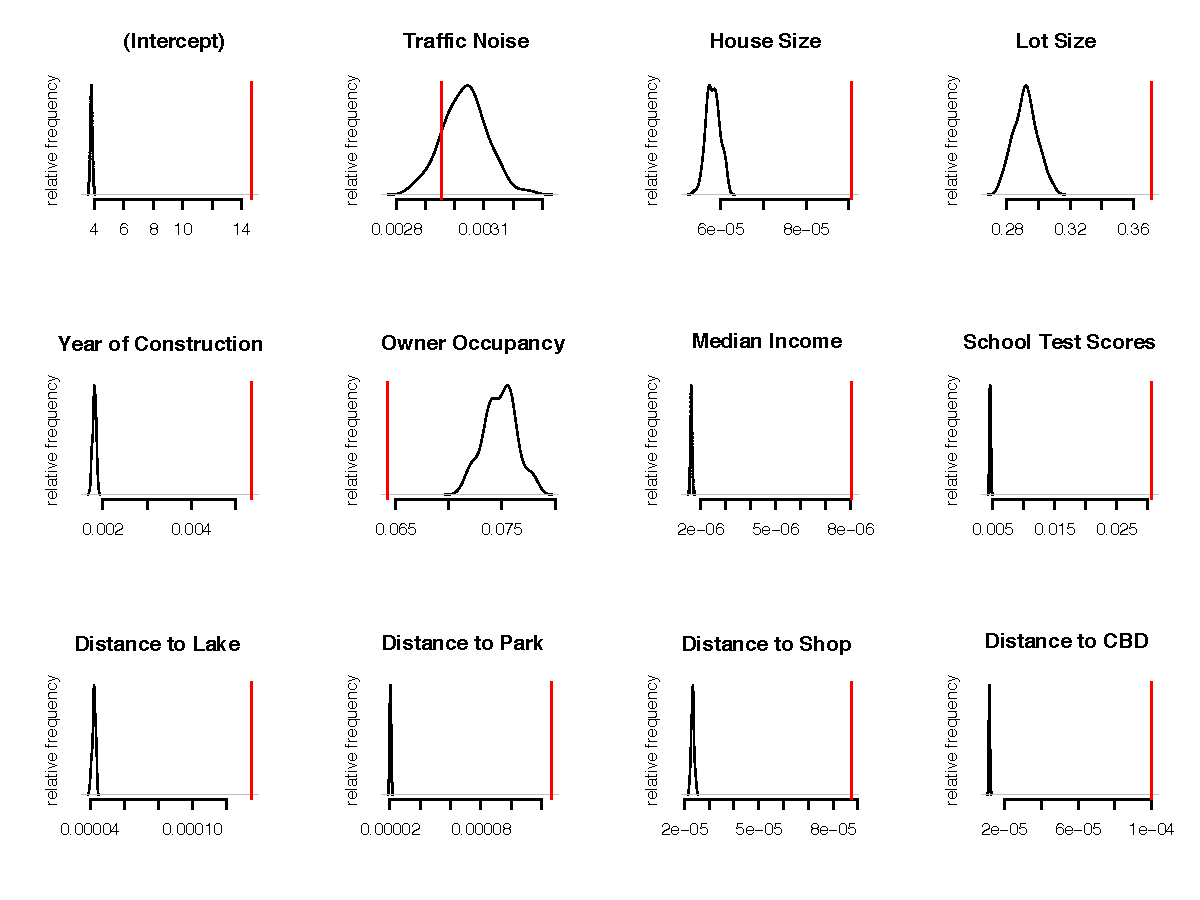
\includegraphics[width=1.2\textwidth]{../graphs/MCsimResultsSDsClean}}
 \caption{Actual LWR Coefficient Standard Deviations \textcolor{red}{(red line)} vs.\ Distribution of Monte Carlo Simulation Standard Deviations by Variable. Figures in which the red line is to the right of the black distribution suggest spatial non-stationarity in effect of the variable on house prices in our study region.}\label{fig:MCsds}
\end{figure}

The results of these simulations suggest that spatial non-stationarity exists in the hedonic function and that LWR techniques are able to capture a significant portion of the non-stationarity. Using a bandwidth of the nearest 200 houses and a temporal lag of 12 months not only yielded significantly smaller GCV scores compared to other bandwidths and model specifications, but such performance does not seem to be a result of a chance spatial arrangement of the data. However, contrary to previous work, these simulations show no evidence for spatial variation in the effect of traffic noise on house prices.

\subsection{Does the Implicit Price of Traffic Noise Change over Time?}

Previous research has suggested that the impact of noise can change with time and economic conditions. For instance, \citet{Wilhelmsson2000} found that the traffic noise penalty to be stronger in the 1990s near Stockholm, Sweden compared to the 1980s. \citet{Cohen2009} also found the (airport) noise penalty to be larger in the early 2000s compared to the late 1990s in Atlanta, Georgia. We know that house prices in the United States fell dramatically during and after the Great Recession of 2008-09. We know less about the patterns of change in the hedonic price functions during and after the fall in house prices. \citet{Cho2011b} found evidence from hedonic analysis in Nashville, Tennessee,  that consumers' willingness to pay for environmental amenities (such as proximity to open space and water views) decreased during the recession as compared to the previous economic boom. 

In this section we look for evidence of temporal non-stationarity in the hedonic coefficient on traffic noise within our data. Specifically, we create two new variables, ``\texttt{months since September 2008}'' and a dummy variable ``\texttt{post}=1'' for all sales after September 2008. We then regress our LWR noise coefficients on these two variables and their interaction term as shown in equation \eqref{eq:LWRinteraction}, 
\begin{equation}\label{eq:LWRinteraction}
\hat{\beta}_{LWR} = \alpha _0 + \alpha _1 \texttt{*Months since Sep. 2008} + \alpha _2  \texttt{*Post} + \alpha _3 \texttt{*Post*Months since Sep. 2008} + \epsilon.
\end{equation}
The results of this regression will help us understand the patterns of change in the implicit price of traffic noise. In particular, $\alpha_1 \neq 0$ suggests a linear temporal trend in the marginal willingness to pay to avoid traffic noise, while $\alpha_2 \neq 0$ suggests that there was a structural break after September 2008, and $\alpha_3 \neq 0$ will imply a change in the temporal trend after September 2008. The linear regression results presented in Table \ref{tab:betaMAX} show that there the estimated LWR coefficients for traffic noise are significantly smaller after September 2008.
\begin{table}
\caption{Dependent Variable = Traffic Noise LWR Coefficients}\label{tab:betaMAX}
\begin{center}
\begin{tabular}{lrrr}
           & Estimate & Std.\ Err. & t-stat  \\  \hline
(Intercept) & -1.7e-03 &  4.1e-05 &  -43.4   \\
Months since Sep 2008       & 6.9e-06 &  2.0e-06  &   3.5    \\
Post        &-8.0e-04 &  7.2e-05  & -11.1    \\
Post*Months since Sep 2008  &-8.9e-05 &  4.5e-06  & -19.7    \\ \hline
\multicolumn{4}{l}{Residual standard error: 0.003} \\
\multicolumn{4}{l}{N = 31,748, R$^2$: 0.093} \\ %,  Adjusted R$^2$: 0.093
%\multicolumn{4}{l}{Signif. codes:  0 ‘***’ 0.001 ‘**’ 0.01 ‘*’ 0.05 ‘.’ 0.1 ‘ ’ 1}
\end{tabular}
\end{center}
\end{table}

The results in Table \ref{tab:betaMAX} contradict the expectation that environmental amenities will ``matter'' less during and after the Great Recession compared to the housing boom. In fact, these results suggest that the penalty for homes exposed to higher levels of traffic noise became more severe. That is, the negative hedonic coefficients on traffic noise got more negative after September 2008.  

\subsection{Are There Threshold Effects of Traffic Noise?}

Some researchers conclude that the semi-elasticity of noise varies with the level of noise \citep{Andersson2010, MarmolejoDuarteCarlos;GonzalezTamez2009, Theebe2004a, Miedema2001, Wilhelmsson2000}, such as a ``threshold''' effect at 70dB \citep{Wilhelmsson2000, Cohen2009}. Other researchers report no evidence of varying impacts at higher or lower noise intensities \citep{Blanco2011, Baranzini2010, Kim2007, Huang;Palmquist2001}. In this section we compare our mean LWR noise coefficient estimates across noise levels to look for threshold effects of traffic noise.

\begin{table}
\begin{center}
\caption{LWR Noise Coefficients vs.\ Noise Levels}\label{tab:LWRnonlinear}
\begin{tabular}{lrrr}
         &   Estimate & Std.\ Err. & t-value \\ \hline
(Intercept) & -1.8e-03 & 1.3e-04  &-13.3 \\
Noise       & -2.8e-06 & 2.3e-06  & -1.2 \\  
Post        & -3.6e-03 & 2.2e-04  &-16.2 \\
Noise*Post  &  3.4e-05 & 4.0e-06  &  8.5 \\ \hline
\multicolumn{4}{l}{Residual standard error: 0.003} \\
\multicolumn{4}{l}{N: 31,748, R$^2$: 0.083} \\
%F-statistic: 961.4 on 3 and 31744 DF,  p-value: < 2.2e-16 
\end{tabular}
\end{center}
\end{table}

Table \ref{tab:LWRnonlinear} reports the results of a simple linear regression of the LWR noise coefficients on the noise levels and whether or not the sale took place before or after September 2008 (as well as their interaction). The table reveals no statistically measurable linear relationship between the noise coefficient and the noise level for sales before September 2008. That is, the semi-elasticity is no different in our data at low levels of noise than at high levels of noise. The positive and significant interaction term suggests that the impact may be different for high vs.\ low levels of noise post-September 2008, but the difference in the predicted marginal effects is so small that it works about to be a roughly \$25 difference for a \$300,000 house at 50 vs.\ 75 dB. Thus, while other researchers report finding impact thresholds at 70dB, we cannot corroborate such findings with our data.

Figure \ref{fig:betaMAXvCat} visually displays the estimated relationship between the level of traffic noise, time, and the estimated LWR traffic noise coefficients. We categorize the traffic noise data in 5 dB wide bins like \citet{Theebe2004a} and then estimate the mean LWR traffic noise coefficients in each category while also controlling for whether the sales took place pre- or post-September 2008. We see little to suggest any meaningful non-linearities in the regression coefficients of traffic noise on house prices, once we have controlled for the timing of the sales.

\begin{figure}
\makebox[\textwidth][c]{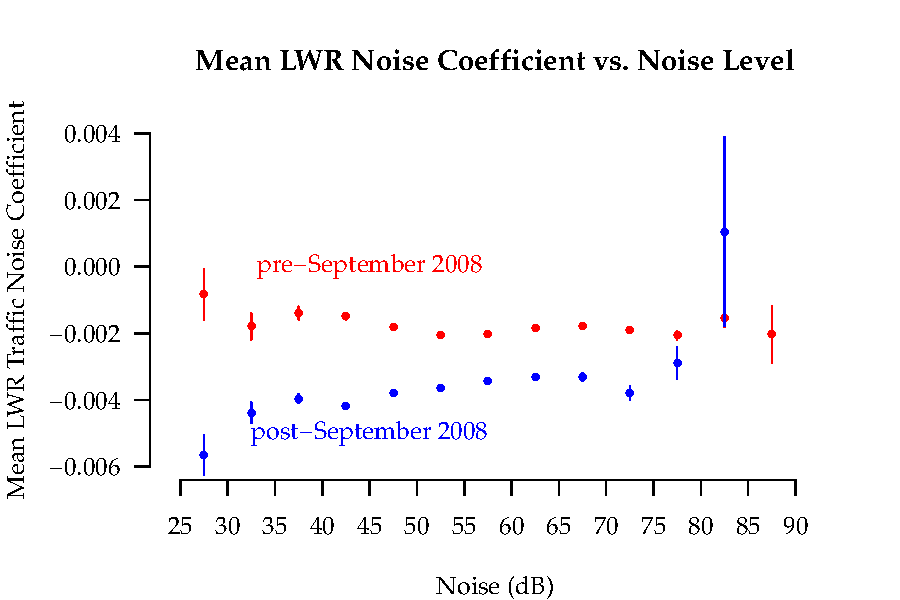
\includegraphics[width = 1.1\textwidth]{../graphs/LWRbetaMAXbyCatTime}}
\caption{The mean LWR traffic noise coefficient by 5 decibel category and pre- vs.\ post-September 2008. The vertical lines denote the standard error of the estimated mean by time and level category. Note that over 99 percent of our data have Noise levels between 35 and 80 dB and no houses were sold post-September 2008 with noise levels above 85 dB.}\label{fig:betaMAXvCat}
\end{figure}


\section{Discussion}\label{Discussion}

The hedonic analysis results presented suggest that traffic noise exhibits a significant negative effect on house prices and that the hedonic function varies over space and time. These results and analysis rest on important assumptions, which if violated, may change the results. This section describes two assumptions that we think are most noteworthy of discussion: lack of omitted variable bias and temporal non-stationarity in the level of several variables across the region during our study period.

Our previously reported results lack some important control variables in the hedonic function. To the extent that structural variables like the number of bedrooms, bathrooms, garage size, or construction quality co-vary with other variables in our dataset, our regression coefficients will suffer from omitted variable bias. We are comforted, however, because we do have some of these important additional variables for a subset of our data. We obtained the number of bedrooms, bathrooms, and garage area for our houses located within Dakota County from the Dakota County Assessor's Office. Our LWR analysis (Models 1, 2, and 3 described earlier) was repeated on this geographic subset of the data and the results were compared to the estimates obtained from the same analysis when these additional structural variables were omitted. We found strikingly similar estimates of the impact of traffic noise suggesting that our results may be robust to the omission of these variables from our analysis.

\begin{table}
\begin{center}
\caption{Noise Coefficient Estimates in Dakota County with and without Additional Structural Variables}\label{tab:Dak}
\begin{tabular}{lll}
 & \multicolumn{2}{p{1.25in}}{Additional Variables Included in LWR?} \\
Locally Weighted Regression Model & \multicolumn{1}{c}{no} & \multicolumn{1}{c}{yes} \\ \cline{1-3}
\multirow{2}{*}{Model (1) = Structural Variables} & -0.0015 & -0.0015 \\ 
   & (0.0023) & (0.0031)  \\[.2cm]
\multirow{2}{*}{Model (2) = Model (1) + Locational Variables} & -0.0014 & -0.0014  \\ 
   & (0.0018) & (0.0022)  \\[.2cm] 
\multirow{2}{*}{Model (3) = Model (2) + City Fixed Effects} & -0.0014 & -0.0014 \\ 
   & (0.0022) & (0.0018) \\[.2cm] \cline{1-3}
\multicolumn{3}{p{4.25in}}{Mean and (standard deviation) LWR traffic noise coefficients when the number of bedrooms, bathrooms, and garage size are included as additional control variables in the regression.}
\end{tabular}
\end{center}
\end{table}

Table \ref{tab:Dak} shows that the traffic noise coefficients estimated by our LWR models are similar regardless of whether the additional structural variables were included or not. Welch two-sample t-tests fail to reject the null hypothesis of zero mean differences across our three models (comparing LWR estimates with vs.\ without the additional structural variables included in the model). Paired t-tests find differences for Model 2 and 3, but the estimated differences are zero to four decimal places and in one case the noise impact estimates with the additional variables are slightly larger and in the other case they are slightly smaller. We also conducted simple linear regressions of the noise coefficients without the additional structural variables on the noise coefficients obtained with the additional structural variables for each of our three models. In all cases the model intercept estimates were close zero, the slopes almost exactly equal to one, and $R^2$ values over 0.7. These results suggest the hedonic coefficients for traffic noise are unaffected by omitted variable bias from common structural variables. While we cannot confirm that this lack of omitted variable bias also occurs elsewhere in our data, the results from Dakota County are promising. 

The timing of our independent variable collection is also a potential weakness. While our house sales data are collected over the course of six years, some of our other variables were collected at specific points in time and assumed to be constant over the study period. In particular, the traffic noise estimates are for the year 2007. To the extent that traffic flows and composition significantly changed over time, our traffic noise variables may be inaccurate for those other time periods. For instance, the US Department of Transportation reports that total vehicle miles traveled decreased by up to 4 percent year-on-year during the Great Recession.\footnote{\url{http://www.fhwa.dot.gov/ohim/tvtw/08dectvt}} Thus, our noise estimates may be inaccurate for later time periods and this may bias our estimates of the impact of noise on house values. Future work may seek to create time-series noise data in order to obtain even better estimates of the impact of traffic noise over time. Given the computational complexity of re-estimating the landscape noise surface, such work is beyond the scope of this paper.

\section{Conclusion}
We estimated the impact of traffic noise on housing prices using Locally Weighted Regression techniques in the St.\ Paul, Minnesota, urban area. Specifically, we estimate semi-logarithmic regressions at each house within our dataset using only information contained in ``local'' (both geographically and temporally) house sales. We find strong evidence that the hedonic function in our study area varies over space and time and such flexible models represent significant improvements over conventional parametric models. 

Monte Carlo simulations suggest that the better goodness-of-fit provided by the local models are not due to chance and that many hedonic implicit prices vary over space within our study area. When the location of our data was randomly assigned and our LWR model was re-estimated across more than a dozen different bandwidths, in 100 consecutive simulations the smallest GCV score was obtained when the data were analyzed at a pooled/global level rather than local. That is, after trying thousands of different combinations of varying levels of local analysis with the spatially redistributed data, we never came close to estimating our observed housing sales prices as well as we can with the local analysis on the actual data. Additionally, re-estimating the LWR model using a local bandwidth of 200 nearest house sales but randomly assigned locations yielded substantially smaller standard deviations for the majority of our regression coefficients. Such differences suggest that the variation exhibited by most of our regression coefficients was not due to simple random chance, but instead is consistent with spatial non-stationarity. 

Contrary to the previous results presented by \citet{MarmolejoDuarteCarlos;GonzalezTamez2009} and \citet{Theebe2004a}, we find little evidence to suggest that the impact of traffic noise varies geographically or by the level of noise within our study area. The traffic noise coefficient was one of only two variables with regression coefficient standard deviations smaller than or similar to the simulated distributions obtained from Monte Carlo experiments. We do, however, find significant temporal variation in the impact of traffic noise in our data. The estimated impact of one additional decibel of traffic noise is a 0.19 percent reduction in the sale price of houses before September 2008, vs.\ 0.37 percent after September 2008. Lastly, after controlling for the Great Recession, we find no significant differences in the impact of traffic noise across the range of commonly seen noise levels (50-70 dB).

Precise estimates of the impact of traffic noise are important for efficient implementation of noise mitigation projects. The US Federal Highway Administration reports that 47 states have constructed noise barriers to reduce noise propagation, spending over a half a billion dollars from 2008-2010 \citepalias{USFHA2012}. \citet{Delucchi1998} used an estimate of 0.85 percent reduction in house prices per additional decibel in their cost-benefit analysis of traffic noise. While their preferred estimate of the total damage cost to the United States in 1991 is \$3 billion, they report a possible range of less than \$100 million to over \$40 billion due in part to uncertainty surrounding the degree of noise propagation over space in the urban built environment and the effect of noise on house prices. Indeed, one of the main conclusions of their work is that more research should be done to better understand the impact of noise on house prices and that better noise data are needed for such work to occur. 

Future research should be conducted in more housing markets, as the potential to apply the results of analysis in one set of geographical and economic circumstances may be limited. Second, ``mixed'' regression techniques (in which some regression coefficients are constrained to remain constant across the study area while others are allowed to vary) may allow researchers to obtain more precise estimates of the impact of hedonic characteristics by increasing the degrees of freedom in the regression. Future work may also seek to re-estimate traffic noise models over time to better account for changes in traffic flows associated with macroeconomic conditions. Lastly, researchers should take advantage of the recent suggestions in \citet{Carruthers2010} and use the spatial variation in regression coefficients obtained from LWR models to estimate the second-stage hedonic regressions to identify consumer demand curves for these characteristics.

\newpage
\begin{singlespace}
\bibliographystyle{plainnat}
\bibliography{NoiseBibliography}
\end{singlespace}
\end{document}

% \begin{table}
% \caption{Data Description}\label{tab:descriptive}
% \begin{tabular}{lp{3in}r}
% Variable & Description  & Expected Hedonic Impact \\ \
% 
% Sale Price &   Price of most recent sale  (in \$) & \\
% 
% Home Size	& Area of finished space in the home (in square feet)	& (+) \\
% Lot Size	& Area of land house sits on (in acres)	& (+) \\
% Year Built & Year home was constructed &	(+) \\
% Owner	Occupancy & Does the owner occupy the house? (0 or 1) &	(+) \\
% 
% Traffic Noise	& Maximum decibel level of traffic noise (dB) measured within parcel &	(-) \\
% MCA 3  & Average 3rd grade Minnesota Comprehensive Assessment (MCA) score for local elementary school &	(+) \\
% Median Income	& Median household income (in dollars) for 2010 Census tract &	(+) \\
% Dist. to CBD &	Distance (in meters) to nearest central business district	& (-) \\
% Dist. to shop &	Distance (in meters) to nearest major shopping center	& (+)/(-) \\
% Dist. to lake &	Distance (in meters) to nearest public lake	& (-) \\
% Dist. to park	& Distance (in meters) to nearest public park	& (-) \\
% City &	City a parcel resides in	& (+)/(-) \\ \hline
% \multicolumn{3}{l}{Total number of house sales between 2005 and 2010 (n = 42,095) }
% \end{tabular}
% \end{table}
